
\begin{frame}
        \frametitle{Auxilliary Activities}

            \begin{figure}[htbp!]
        \begin{center}
          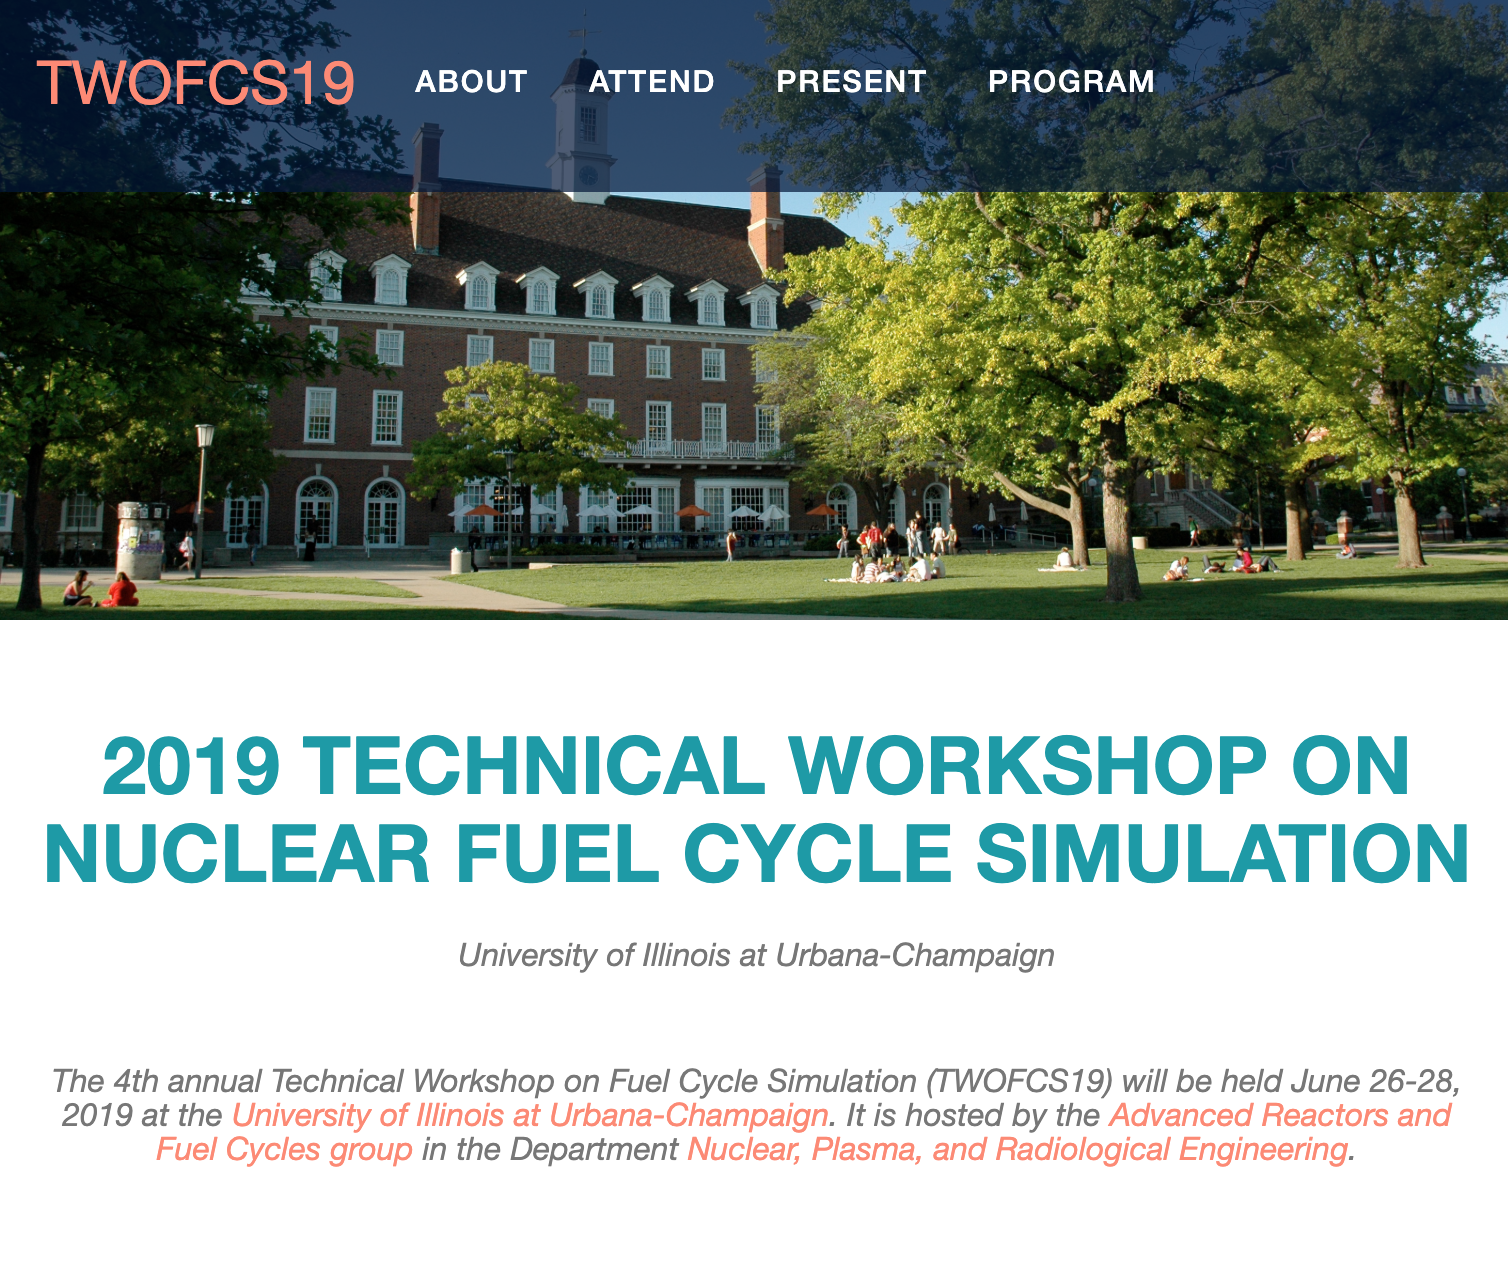
\includegraphics[width=0.8\textwidth]{images/twofcs.png}
        \end{center}
              \caption{Technical Workshop, not funded by DOE, but well attended 
                    by DOE SA\&I community.}
      \end{figure}
\end{frame}

\begin{frame}
        \frametitle{Auxilliary Activities}


        Cyclus (particularly Wisconsin) is a key participant in the 
        Functionality Isolation Test Benchmark.
        \begin{itemize}
             \item CNRS / IN2P3 (Xavier Doligez, Marc Ernoult and Nicolas Thiollière) - CLASS
             \item University of Wisconsin - Madison (Paul Wilson and Baptiste Mouginot) - CYCLUS
             \item University of South Carolina (Robert Flanagan) - CYCLUS
             \item University of Illinois at Urbana-Champaign (Katy Huff) - CYCLUS
             \item Argonne National Lab (Bo Feng) - DYMOND
             \item Oak Ridge National Lab (Eva E. Davidson) - ORION
             \item Idaho National Lab (Ross Hays) - VISION
             \item CIEMAT (Aris Villacorta, Fransisco Alvarez) - Tr\_Evol / 
                     Evol\_code
             \item TRACTEBEL (Hubert Druenne, Bart Vermeeren) - ANICCA
             \item Univ. of technology and economics of Budapest (Mate Halasz, Màté Szieberth) - SITON
             \item Hungarian Academy of Sciences (Aron Brolly) - SITON
             \item Universidad Católica del Maule (Ivan Merino) - ANICCA
        \end{itemize}
\end{frame}
